\section{FrBu II.2 2}

\questionBox{
    Let $\alpha : [0, \pi] \rightarrow \mathbb{C} $ be defined by
    $$\alpha(t) = e^{it}$$
    and $\beta : [0, 2] \rightarrow \mathbb{C} $ by

    \[
        \beta(t)=\left\{
        \begin{array}{lll}
            1 + t(-i-1) & \text{for } t \in [0,1]\\
            1 - t +i(t-2) & \text{for } t \in [1,2].
        \end{array}
        \right.
    \]

    Sketch $\alpha$, and $\beta$, and calculate

    $$ \int_{\alpha} \frac{1}{z} dz \text{ and } \int_{\beta} \frac{1}{z} dz.$$
}

\answerBox{
Sketch of $\alpha$, and $\beta$:

\begin{figure}[H]
    \centering
    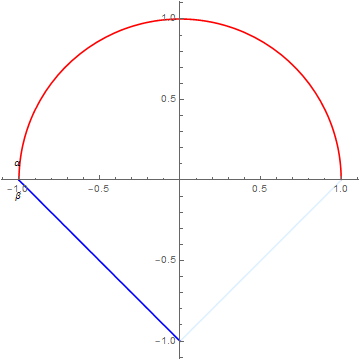
\includegraphics[width=0.5\textwidth]{pics/frbu212.png}
%   \caption{}
\end{figure}

Calculation of the integral along $\alpha$:
\begin{alignat*}{2}
    \int_{\alpha} \frac{1}{z} dz &= \int_{0}^{\pi} \frac{1}{e^{it}}i e^{it} dt &\qquad\hyperref[sec:ContourIntegral]{(1)} \\
    & = \int_{0}^{\pi} i dt & \\
    & = \left[ i t \right]_0^\pi & \\
    & = \pi i &
\end{alignat*}

Calculation of the integral along $\beta$:
\begin{equation*}
    \begin{split}
        \int_{\beta} \frac{1}{z} dz &= \int_0^1 \frac{-i-1}{1+t (-i-1)} \, dt+\int_1^2 \frac{-1+i}{1-2 i+t (-1+i)} \, dt \\
        & = \left[ \log (-1+(1+i) t) \right]_0^1 + \left[ \log ((-2-i)+(1+i) t) \right]_1^2 \\
        & = -\pi i
    \end{split}
\end{equation*}
}